% Fig. 1 of the paper (method overview and toy run), as a standalone TikZ file.
% Build: pdflatex fig1_overview.tex   (no data input; "(2)" is the bracket test, Eq. 2 of the paper)
\documentclass[border=2pt,varwidth=12.2cm]{standalone}
\usepackage[T1]{fontenc}
\usepackage{amsopn}
\usepackage{tikz}
\usetikzlibrary{positioning,arrows.meta}
\begin{document}
\centering
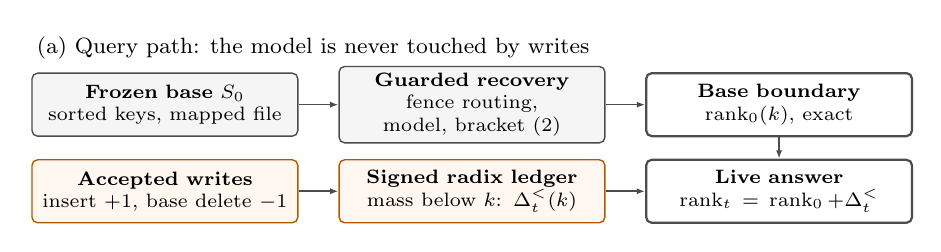
\begin{tikzpicture}[
  font=\scriptsize,
  bx/.style={draw,rounded corners=2pt,line width=.5pt,text width=3.2cm,align=center,inner sep=2.5pt,minimum height=0.8cm},
  bs/.style={bx,draw=black!70,fill=black!4},
  ld/.style={bx,draw=orange!70!black,fill=orange!6},
  rs/.style={bx,draw=black!70,fill=white,line width=.8pt},
  fl/.style={-{Latex[length=3pt]},line width=.6pt,black!70}]
\node[bs] (s0) at (0,0) {\textbf{Frozen base $S_0$}\\sorted keys, mapped file};
\node[bs] (rc) at (3.9,0) {\textbf{Guarded recovery}\\fence routing, model, bracket~(2)};
\node[rs] (r0) at (7.8,0) {\textbf{Base boundary}\\$\operatorname{rank}_0(k)$, exact};
\node[ld] (wr) at (0,-1.1) {\textbf{Accepted writes}\\insert $+1$, base delete $-1$};
\node[ld] (lg) at (3.9,-1.1) {\textbf{Signed radix ledger}\\mass below $k$: $\Delta^{<}_t(k)$};
\node[rs] (rt) at (7.8,-1.1) {\textbf{Live answer}\\$\operatorname{rank}_t=\operatorname{rank}_0+\Delta^{<}_t$};
\draw[fl] (s0)--(rc); \draw[fl] (rc)--(r0); \draw[fl] (wr)--(lg); \draw[fl] (lg)--(rt); \draw[fl] (r0)--(rt);
\node[anchor=west,font=\footnotesize] at (-1.75,0.72) {(a) Query path: the model is never touched by writes};
\end{tikzpicture}\\[6pt]
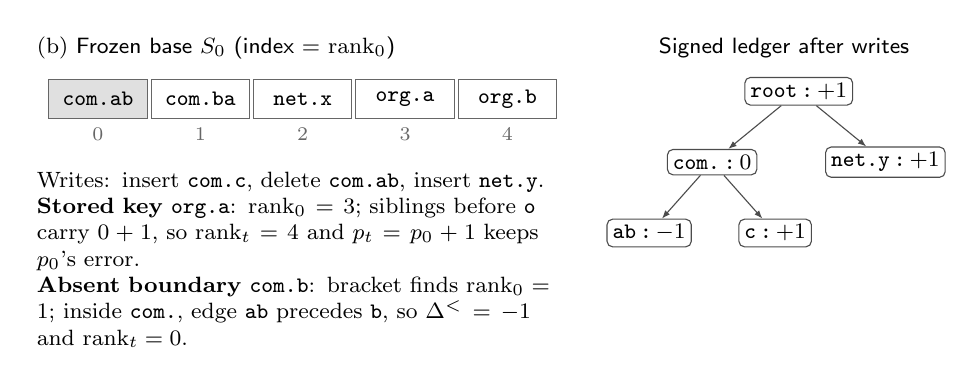
\begin{tikzpicture}[
  font=\footnotesize,
  cell/.style={draw=black!60,minimum width=1.25cm,minimum height=.5cm,inner sep=1pt,font=\ttfamily\footnotesize},
  gone/.style={cell,fill=black!12},
  tn/.style={draw=black!70,rounded corners=2pt,inner sep=2pt,font=\ttfamily\footnotesize},
  ed/.style={-{Latex[length=3pt]},black!70}]
\node[anchor=west] at (-0.9,0.9) {(b) \textsf{Frozen base $S_0$ (index = $\operatorname{rank}_0$)}};
\foreach \s/\n [count=\i from 0] in {com.ab/gone,com.ba/cell,net.x/cell,org.a/cell,org.b/cell}{
  \node[\n] (b\i) at (\i*1.3,0.25) {\s};
  \node[font=\scriptsize,black!60] at (\i*1.3,-0.2) {\i};}
\node[anchor=west] at (7.0,0.9) {\textsf{Signed ledger after writes}};
\node[tn] (r) at (8.9,0.35) {root\,:\,$+1$};
\node[tn] (c) at (7.8,-0.55) {com.\,:\,$0$};
\node[tn] (n) at (10.0,-0.55) {net.y\,:\,$+1$};
\node[tn] (a) at (7.0,-1.45) {ab\,:\,$-1$};
\node[tn] (cc) at (8.6,-1.45) {c\,:\,$+1$};
\draw[ed] (r)--(c); \draw[ed] (r)--(n); \draw[ed] (c)--(a); \draw[ed] (c)--(cc);
\node[anchor=north west,align=left,text width=6.6cm] at (-0.9,-0.55) {%
Writes: insert \texttt{com.c}, delete \texttt{com.ab}, insert \texttt{net.y}.\\
\textbf{Stored key} \texttt{org.a}: $\operatorname{rank}_0=3$; siblings before \texttt{o} carry $0+1$, so $\operatorname{rank}_t=4$ and $p_t=p_0+1$ keeps $p_0$'s error.\\
\textbf{Absent boundary} \texttt{com.b}: bracket finds $\operatorname{rank}_0=1$; inside \texttt{com.}, edge \texttt{ab} precedes \texttt{b}, so $\Delta^{<}=-1$ and $\operatorname{rank}_t=0$.};
\end{tikzpicture}
\end{document}
